\documentclass[tikz,border=6pt]{standalone}
\usepackage[T1]{fontenc}
\usepackage{lmodern}
\usepackage{amsmath}
\usepackage{amssymb}
\usepackage{bm}
\usepackage{xcolor}
\usepackage{tikz}
\usetikzlibrary{arrows.meta,positioning,fit,calc,backgrounds,shapes.multipart,shapes.geometric}

\colorlet{mandalaBlue}{blue!55!black}
\colorlet{mandalaTeal}{teal!55!black}
\colorlet{mandalaGreen}{green!45!black}
\colorlet{mandalaGold}{orange!70!black}
\colorlet{mandalaRed}{red!55!black}
\colorlet{mandalaViolet}{violet!55!black}
\colorlet{mandalaGray}{black!55}
\colorlet{mandalaLight}{black!3}

\tikzset{
  >=Latex,
  font=\sffamily,
  % Color semantics used consistently across all diagrams:
  % mandalaBlue   -> external inputs / sources / configuration
  % mandalaTeal   -> internal data containers / encoded features
  % mandalaGreen  -> geometric or physics-aware transformations
  % mandalaGold   -> model computation or linear-algebra solve stages
  % mandalaViolet -> predicted operator-valued objects and heads
  % mandalaRed    -> optimization / objectives / losses
  titlebox/.style={
    rounded corners=2.5pt,
    fill=mandalaBlue!8,
    draw=mandalaBlue,
    line width=0.8pt,
    inner sep=6pt,
    minimum height=10mm,
    align=center,
    font=\sffamily\bfseries\large
  },
  panel/.style={
    rounded corners=3pt,
    fill=white,
    draw=black!45,
    line width=0.8pt,
    inner sep=5pt
  },
  stage/.style={
    rounded corners=3pt,
    fill=#1!10,
    draw=#1!85!black,
    line width=0.9pt,
    minimum width=32mm,
    minimum height=11mm,
    align=center,
    font=\sffamily\small
  },
  stage/.default=mandalaBlue,
  smallstage/.style={
    rounded corners=2.5pt,
    fill=#1!9,
    draw=#1!80!black,
    line width=0.75pt,
    minimum width=27mm,
    minimum height=8.5mm,
    align=center,
    font=\sffamily\scriptsize
  },
  smallstage/.default=mandalaBlue,
  sidepanel/.style={
    rounded corners=3pt,
    fill=#1!8,
    draw=#1!75!black,
    line width=0.8pt,
    inner sep=5pt,
    align=left,
    font=\sffamily\scriptsize,
    text width=43mm
  },
  sidepanel/.default=mandalaTeal,
  annot/.style={
    font=\sffamily\scriptsize,
    text=mandalaGray,
    align=left
  },
  arrow/.style={
    -{Latex[length=2.6mm,width=1.8mm]},
    line width=0.95pt,
    draw=black!70
  },
  dashedarrow/.style={
    -{Latex[length=2.4mm,width=1.7mm]},
    line width=0.85pt,
    draw=black!65,
    dashed
  },
  softfit/.style={
    rounded corners=4pt,
    draw=black!35,
    fill=black!1,
    line width=0.7pt,
    inner sep=6pt
  },
  lab/.style={
    font=\sffamily\scriptsize\bfseries,
    text=black!75
  },
  tinycode/.style={
    font=\ttfamily\tiny,
    text=black!70,
    align=center
  }
}

\begin{document}
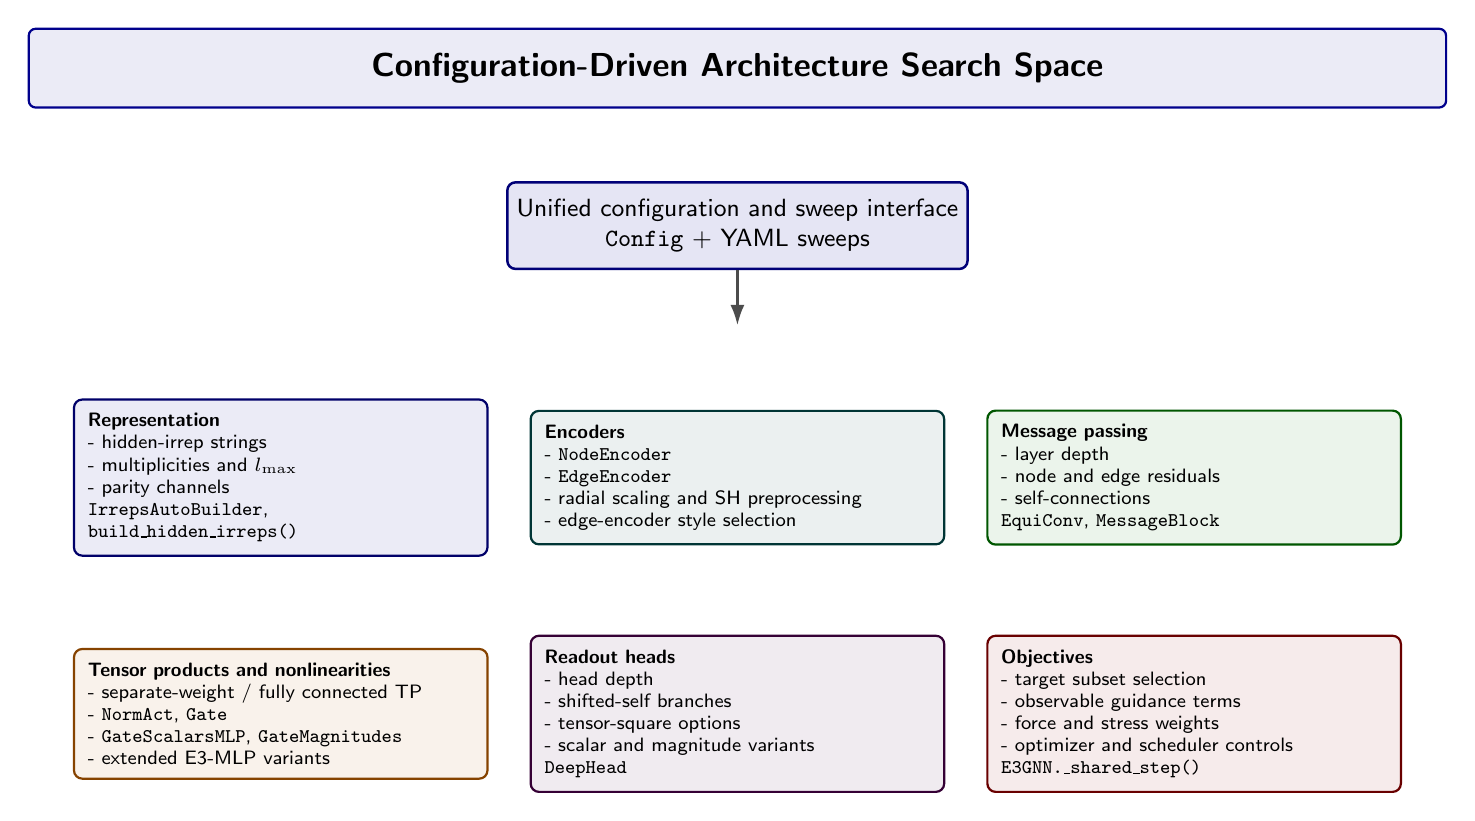
\begin{tikzpicture}[x=1cm,y=1cm]

\node[titlebox, minimum width=18.0cm] (title) at (0,0) {Configuration-Driven Architecture Search Space};

\node[stage=mandalaBlue, minimum width=5.0cm] (cfg) at (0.0,-2.0)
{Unified configuration and sweep interface\\
\texttt{Config} + YAML sweeps};

\draw[arrow] (cfg.south) -- +(0,-0.7);

\node[sidepanel=mandalaBlue, text width=4.9cm] (rep) at (-5.8,-5.2)
{\textbf{Representation}\\
- hidden-irrep strings\\
- multiplicities and $l_{\max}$\\
- parity channels\\
\texttt{IrrepsAutoBuilder}, \texttt{build\_hidden\_irreps()}};

\node[sidepanel=mandalaTeal, text width=4.9cm] (enc) at (0.0,-5.2)
{\textbf{Encoders}\\
- \texttt{NodeEncoder}\\
- \texttt{EdgeEncoder}\\
- radial scaling and SH preprocessing\\
- edge-encoder style selection};

\node[sidepanel=mandalaGreen, text width=4.9cm] (mp) at (5.8,-5.2)
{\textbf{Message passing}\\
- layer depth\\
- node and edge residuals\\
- self-connections\\
\texttt{EquiConv}, \texttt{MessageBlock}};

\node[sidepanel=mandalaGold, text width=4.9cm] (tp) at (-5.8,-8.2)
{\textbf{Tensor products and nonlinearities}\\
- separate-weight / fully connected TP\\
- \texttt{NormAct}, \texttt{Gate}\\
- \texttt{GateScalarsMLP}, \texttt{GateMagnitudes}\\
- extended E3-MLP variants};

\node[sidepanel=mandalaViolet, text width=4.9cm] (head) at (0.0,-8.2)
{\textbf{Readout heads}\\
- head depth\\
- shifted-self branches\\
- tensor-square options\\
- scalar and magnitude variants\\
\texttt{DeepHead}};

\node[sidepanel=mandalaRed, text width=4.9cm] (obj) at (5.8,-8.2)
{\textbf{Objectives}\\
- target subset selection\\
- observable guidance terms\\
- force and stress weights\\
- optimizer and scheduler controls\\
\texttt{E3GNN.\_shared\_step()}};

\end{tikzpicture}
\end{document}
